%% Copernicus Publications Manuscript Preparation Template for LaTeX Submissions
%% ---------------------------------
%% This template should be used for copernicus.cls
%% The class file and some style files are bundled in the Copernicus Latex Package, which can be downloaded from the different journal webpages.
%% For further assistance please contact Copernicus Publications at: production@copernicus.org
%% https://publications.copernicus.org/for_authors/manuscript_preparation.html


%% Please use the following documentclass and journal abbreviations for preprints and final revised papers.

%% 2-column papers and preprints
\documentclass[hess, manuscript]{copernicus}
\usepackage[compatibility=false]{caption}

%% Journal abbreviations (please use the same for preprints and final revised papers)
% Hydrology and Earth System Sciences (hess)


%% \usepackage commands included in the copernicus.cls:
%\usepackage[german, english]{babel}
\usepackage{tabularx}
%\usepackage{cancel}
%\usepackage{multirow}
%\usepackage{supertabular}
%\usepackage{algorithmic}
%\usepackage{algorithm}
%\usepackage{amsthm}
%\usepackage{float}
%\usepackage{subfig}
%\usepackage{rotating}
\usepackage{booktabs}


\begin{document}

\title{Benchmarking reservoir operation schemes for large-scale hydrological models}


% \Author[affil]{given_name}{surname}

\Author[1, 2][j.casado@kajoservices.com]{Jesús}{Casado-Rodríguez} %% correspondence author
\Author[3]{Juliana}{Disperati}
\Author[1]{Stefania}{Grimaldi}
\Author[1]{Peter}{Salamon}

\affil[1]{European Commission - Joint Research Centre, Ispra (Italy)}
\affil[2]{Kajo s.r.o., Sládkovičova (Slovakia)}
\affil[3]{Fincons Group, Vimercate (Italy)}

%% The [] brackets identify the author with the corresponding affiliation. 1, 2, 3, etc. should be inserted.

%% If an author is deceased, please add \deceased[$Deceased date if applicable$]{$Author number$} (e.g. \deceased[13 November 2015]{2}) at the end of the affiliations. The author number depends on the placement of the author in the author list, e.g. the third author has number 3.


%% If authors contributed equally, please add \equalcontrib{$Author numbers$} (e.g. \equalcontrib{1,3}) at the end of the affiliations. The author number depends on the placement of the author in the author list, e.g. the third author has number 3.




\runningtitle{TEXT}

\runningauthor{TEXT}





\received{}
\pubdiscuss{} %% only important for two-stage journals
\revised{}
\accepted{}
\published{}

%% These dates will be inserted by Copernicus Publications during the typesetting process.


\firstpage{1}

\maketitle



\begin{abstract}
There are approximately 62,000 large dams worldwide that significantly alter the hydrological regimes of most major rivers. Despite their importance, reservoirs remain poorly represented in Large-Scale Hydrological Models (LSHMs) due to the complexity of human-driven operations and a widespread lack of observational records. Consequently, reservoir routines in LSHMs must balance structural simplicity with limited data requirements. In this study, we utilize the ResOpsUS dataset to benchmark four reservoir routines of increasing complexity: LISFLOOD, CaMa-Flood, mHM, and STARFIT. We evaluate these routines across 164 reservoirs in the United States and test which target variables are most informative for parameter estimation. Our results indicate that the mHM routine consistently achieves the highest performance; however, its dependence on site-specific demand data limits its applicability at the global scale. In contrast, the CaMa-Flood routine provides a robust compromise, significantly outperforming the linear logic of LISFLOOD while maintaining parsimonious data requirements. Crucially, we find that calibrating to reservoir storage is more informative than calibrating to outflow, as it effectively captures the dynamics of both state variables. This finding paves the way for the use of satellite-derived storage products in the calibration of LSHMs. The findings of this study have been implemented in the upcoming versions of the European and Global Flood Awareness Systems (EFAS v6 and GloFAS v5).
\end{abstract}


%\copyrightstatement{TEXT} %% This section is optional and can be used for copyright transfers.


\introduction 

% Reservoir impacts: number and capacity, alteration of the water cycle, difficulties in forecasting discharge
%\citep{Wisser2010, Biemans2011, Scherer2016, Salwey2023, Moreno-Rodenas2025, Mulligan2020, Wang2022, ICOLD2024, Doll2009, Zhou2016}

The increasing global population and expanding economic activities have amplified the pressure on freshwater resources, making human interventions—such as the construction and operation of dams and reservoirs—fundamental elements of the terrestrial water cycle \citep{Biemans2011, Busker2019, Moreno-Rodenas2025, Sadki2023}. These structures are pivotal in fulfilling diverse societal needs, including domestic and industrial water supply, irrigation, hydropower production, and flood control \citep{Moreno-Rodenas2025, Abeshu2023, Lehner2024, Mekonnen2012, Sadki2023, Shrestha2024}. The global proliferation of dams has been unprecedented over the last century \citep{Lehner2024, Moreno-Rodenas2025}. Globally, there are approximately 62,000 large dams (heights > 15 m), cataloged by the ICOLD (International Commission on Large Dams)  \citep{Moreno-Rodenas2025}, with an estimated cumulative storage capacity ranging between 7,420 $\text{km}^3$  (GDW v1.0) \citep{Lehner2024} and 8,300 $\text{km}^3$ \citep{Sadki2023}. This volume represents roughly 20\% of the average annual river discharge to the oceans and is four times the amount of water stored in river channels worldwide \citep{Sadki2023}.

The immense scale of this intervention profoundly impacts natural hydrology by modifying the magnitude, timing, and duration of streamflows \citep{Salwey2024, Shin2019}, resulting in the fragmentation of over 60\% of the world's largest rivers \citep{Sadki2023}. In the contiguous United States (CONUS), dams regulate all major rivers, providing a total storage capacity equivalent to roughly 75\% of the mean annual CONUS runoff \citep{Steyaert2022}. While beneficial for human use, these operations cause significant environmental trade-offs, including the homogenization of river dynamics \citep{Lehner2024, Scherer2016}, alteration of sediment and nutrient transport \citep{Shin2019, Yassin2019}, and increased open-water evaporation, which can exacerbate water scarcity \citep{Yassin2019, Scherer2016}.

% Different model perspectives
%\citep{Abeshu2023, Coerver2018, Hanasaki2006, Hanazaki2022, Sadki2023, Shin2019, Shrestha2024, Turner2021, Steyaert2025, Yassin2019}
Despite their importance, the accurate representation of complex reservoir operations remains a challenge in large-scale hydrological models (LSHMs) and land-surface models (LSMs) \citep{Sadki2023, Salwey2024, Turner2021}. Reservoir operations are intrinsically non-linear and governed by complex, human-driven decisions related to water demand, flood risk, and environmental constraints \citep{Shrestha2024, Coerver2018, Hanazaki2022, Salwey2024, Steyaert2022}. Consequently, models lacking adequate reservoir schemes often exhibit degraded predictive performance, especially in highly regulated basins \citep{Salwey2024, Turner2021, Steyaert2025}. Historically, global models have relied on generic operational rules utilizing static characteristics (e.g., capacity, primary purpose) from datasets like the Global Reservoir and Dam (GRanD) database \citep{Lehner2011}. However, these generic approaches often fail to capture the local operating behaviors necessary for simulating realistic daily releases and storage dynamics \citep{Turner2021}. Recent research has therefore pivoted toward exploiting newly available observational data and integrating data-driven techniques, such as machine learning or statistically inferred policies, to better reflect historical decision-making \citep{Turner2021, Coerver2018, Steyaert2025}.

% Introduction to GloFAS and the need for  better reservoir representation
% challenge: global applicability
% challenge: lack of observed data -> ResOpsUS, GRanD/GDW

This research aims to improve the reservoir module within the LISFLOOD hydrological model \citep{DeRoo2000, vanderKnijff2010, Burek2013a}, a core component of the Global and European Flood Awareness Systems (GloFAS and EFAS) \citep{GloFAS2025, EFAS2025}. Current LISFLOOD parameterizations typically employ a single general reservoir operation scheme based on three fixed storage limits (minimum, normal, and non-damaging outflow) without explicit classification of reservoir purpose  \citep{Zajac2017}. Our objective is to identify a reservoir routine suitable for global application—one that balances portability with efficacy in data-scarce environments.

Specifically, this study benchmarks the performance of four distinct methodologies—ranging from classical parameterizations to data-driven approaches—against observed records. The methodologies include the current LISFLOOD parameterization, a recently published evolution (CaMa-Flood), a demand-driven approach (mHM), and a seasonality-driven approach (STARFIT). By assessing their capability to simulate observed flow regulation and storage dynamics, this research provides critical guidance for the selection and development of human-water interaction modules in the next generation of operational flood systems and large-scale hydrological models. 

A novel aspect of this study is the exploration of a decoupled calibration strategy. Rather than calibrating reservoir parameters simultaneously with the rest of the hydrological model against downstream river discharge—a process often plagued by equifinality \citep{Beven2001}—we define reservoir parameters in advance using specific reservoir records. These pre-determined parameters are then integrated into the hydrological model for the subsequent calibration of the remaining parameters. This approach ensures that reservoir parameters are sensitive to actual reservoir dynamics rather than being masked by gauge observations far downstream.

However, the practical implementation of this strategy faces a significant data bottleneck. Often, river discharge in gauging stations downstream the reservoir has been used as the variable informing about reservoir operations. While ground-based records or reservoir outflow provide a more direct target, this data is frequently inaccessible or classified as private. To overcome these limitations, satellite-derived products offer a promising alternative \citep{Pekel2016, Schwatke2015, Schwatke2020, Donchyts2022, Khandelwal2022, Hou2024}.  These products offer the potential to monitor volume fluctuations in ungauged regions, making them crucial for future global model calibration and data assimilation. 

A calibration based on satellite products would target reservoir level or storage, instead of outflow (or river discharge as a proxy variable). To assess the feasibility of using satellite products, we compare the performance of the model when calibrated against three distinct targets: (i) reservoir release only, (ii) reservoir storage only, and (iii) a combined objective function utilizing both variables. By evaluating these configurations, this study aims to assess whether satellite-inferred storage can serve as a robust alternative to ground-based outflow records, thereby enabling improved reservoir modeling in ungauged or data-scarce regions. 

% mention difficulties in accessing ground-based data
% \citep{Zhou2016}
% \citep{Steyaert2025}
The benchmarking is supported by the ResOpsUS dataset \citep{Steyaert2022, Steyaert2024}, the first comprehensive, national-scale inventory providing historical daily reservoir operations for 679 major dams across the CONUS. ResOpsUS includes records of reservoir inflow, level, storage and outflow (not all variables for all reservoirs), providing the necessary variables for our benchmark. We leverage this data-rich environment to test the models and calibration targets, establishing a proof-of-concept for operational environments where such granular data is unavailable.

In summary, this study benchmarks four reservoir modeling paradigms across the CONUS domain to address three primary objectives: (i) to identify the most robust reservoir routine for the next operational versions of GloFAS and EFAS; (ii) to determine the most suitable target variable for calibration—storage, outflow, or both; and (iii) to evaluate whether remotely sensed storage fluctuations are sufficiently informative to calibrate large-scale models.

% Missing:
% * The regionalization approach
 
%\cite{Hanasaki2006} \cite{Haddeland2006} \cite{Abeshu2023}

\section{Data}
\label{sec:data}

\subsection{Reservoir Selection and Filtering}
\label{sec:reservoir_selection}

To evaluate reservoir routines in a data-rich context, we utilized the ResOpsUS dataset \citep{Steyaert2022, Steyaert2024}, which provides daily time series of reservoir operations for 679 reservoirs across the conterminous United States (CONUS). From this initial pool, we applied a rigorous filtering process to ensure the suitability of the reservoirs for large-scale hydrological modeling:

\begin{enumerate}
    \item Data Availability: We selected only those reservoirs containing concurrent daily records for all three primary variables: inflow ($I$), storage ($V$), and outflow ($Q$).
    \item Physical Dimensions: Reservoirs were required to have a minimum catchment area of 50~km² and a minimum storage capacity ($V_{max}$) of 10~hm³.
    \item Hydrological Impact: Following \citet{Shrestha2024}, we excluded "non-disruptive" reservoirs—those that do not significantly alter the natural flow regime. This was quantified using the Degree of Regulation ($\text{DOR}$; Eq.~\ref{eq:degree_of_regulation}) and the Degree of Disruptivity ($\text{DOD}$; Eq.~\ref{eq:degree_of_disruptivity}). Reservoirs with $\text{DOR} < 0.08$ or $\text{DOD} < 0.06$~m were discarded:
    \begin{equation}
        \label{eq:degree_of_regulation}
        \text{DOR} = \frac{V_{max}}{\bar{I}_{yr}} \quad [-]
    \end{equation}
    \begin{equation}
        \label{eq:degree_of_disruptivity}
        \text{DOD} = \frac{V_{max}}{A_c} \quad [\text{m}]
    \end{equation}
    where $V_{max}$ is the reservoir storage capacity [m$^3$], $\bar{I}_{yr}$ is the average annual inflow [m$^3$/year], and $A_c$ is the catchment area [m$^2$].
    \item Record Length: To ensure sufficient data for robust model calibration, we removed reservoirs with time series shorter than four years.
    \item Water Balance Integrity: Preliminary analysis revealed large biases between average inflow and outflow in several reservoirs. Such discrepancies may stem from poor data quality or significant consumptive use (e.g., water diversions) not explicitly represented in our modeling framework. To ensure a closed water balance for benchmarking, we removed reservoirs where the absolute bias exceeded 30\%.
\end{enumerate}

Applying these criteria resulted in a final selection of 164 reservoirs. Their geographical distribution, categorized by catchment area and storage capacity, is depicted in Fig.~\ref{fig:map_reservoirs}.

\begin{figure*}
    \centering
    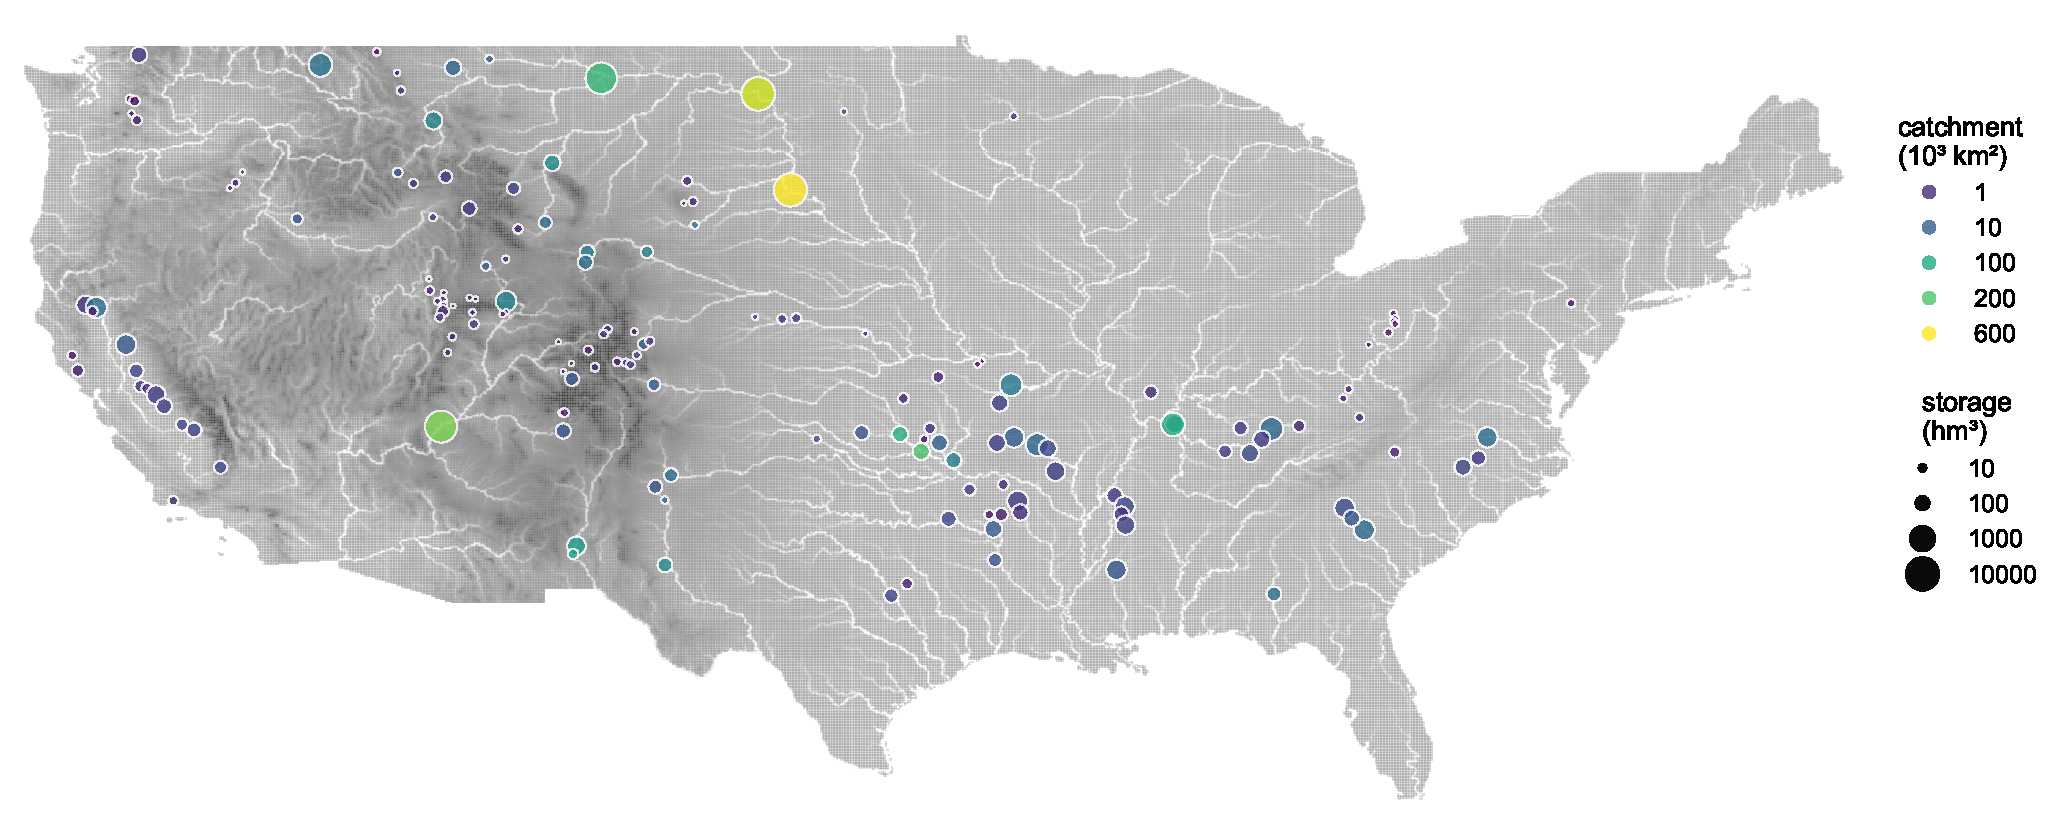
\includegraphics[width=1\textwidth]{figures/figure1.pdf}
    \caption{Distribution of the 164 reservoirs from the ResOpsUS dataset used in the benchmarking. Colors represent the catchment area and point size represents the storage capacity.}
    \label{fig:map_reservoirs}
\end{figure*}

\subsection{Dataset Integration and Attribute Enrichment}
\label{sec:reservoir_attributes}

To satisfy the input requirements of the diverse reservoir routines, we enriched the ResOpsUS records with supplementary hydrometeorological time series, and catchment and reservoir attributes.

As detailed in Sect.~\ref{sec:reservoir_models}, the routines require time series of direct precipitation and evaporation. These were extracted for each reservoir location from the ERA5 reanalysis dataset \citep{Hersbach2020}. 

Static reservoir and dam attributes were primarily sourced from the Global Reservoir and Dam dataset (GRanD) \citep{Lehner2011}. While we included all GRanD attributes in our dataset, four were critical for the simulations: storage capacity ($V_{max}$), maximum surface area ($A_{max}$), dam crest elevation ($Z_{max}$), and dam height ($H_{dam}$). A comparison of these attributes against observed time series revealed inconsistencies in some attribute values. To rectify this, we cross-referenced GRanD with the Global Dam Watch (GDW) dataset \citep{Lehner2024}. For instances where the attributes remained inconsistent, we manually updated the records using official data from U.S. authorities, including the U.S. Army Corps of Engineers' National Inventory of Dams (NID), the U.S. Bureau of Reclamation (USBR), and the U.S. Geological Survey (USGS) \citep{NID, USBR, USGS}. Similar errors were reported by \citet{Shrestha2024}.

For the purpose of parameter regionalization or the development of data-driven models, we further included catchment-scale characteristics derived from GloFAS surface fields \citep{Choulga2024} and climate indices derived from ERA5 \citep{Hersbach2020}. 

We named the enriched dataset \textit{Reservoir Operations US and CAtchment and Reservoir Static attributes} (ResOpsUS+CARS). It is available via \href{https://doi.org/10.5281/zenodo.15978041}{Zenodo}. The dataset structure follows the standards defined by the CARAVAN initiative \citep{Kratzert2023}, ensuring it is formatted for immediate use in deep learning and large-sample hydrological studies.

\section{Methods}
\label{sec:methods}

\subsection{Reservoir models}
\label{sec:reservoir_models}

Each of the reservoir routines evaluated in this study is governed by the water mass balance equation (Eq.~\ref{eq:mass_balance}). At each time step $\Delta t$, the model calculates the reservoir storage at the end of the interval ($V_{t+1}$) based on the preceding storage state ($V_t$), the water surface area ($A_t$), and three forcing variables: inflow ($I_t$), precipitation ($P_t$), and evaporation ($E_t$):

\begin{equation}
    \label{eq:mass_balance}
    V_{t+1} = V_t + \left( P_t - E_t \right) \cdot A_t + \left( I_t - Q_t \right) \cdot \Delta t 
\end{equation}

where $Q_t$ is the reservoir outflow (release), the fundamental difference between the four reservoir schemes. 

To represent the reservoir's bathymetry, we assume a simplified triangular pyramid geometry, following the approach of \citet{Liebe2005} and subsequent studies \citep{Shin2019, Sadki2023, Shrestha2024}.This geometric approximation allows for the continuous estimation of the water surface area (Eq.~\ref{eq:area}), which is required for the mass balance, and the water level ($Z_t$; Eq.~\ref{eq:level}), provided that the dam crest elevation ($Z_{max}$) and the dam height ($H_{dam}$) are known. We evaluate the validity of this geometric assumption by comparing simulated levels against observed records in a subset of reservoirs where such data is available.

\begin{equation}
    \label{eq:area}
    A_t = A_{max} \left(  \frac{V_t}{V_{max}} \right)^{\frac{2}{3}}
\end{equation}
\begin{equation}
    \label{eq:level}
    \begin{aligned}
        h_t &= H_{dam} \left(  \frac{V_t}{V_{max}} \right)^{\frac{1}{3}} \\
        Z_t &= Z_{max} - H_{dam} + h_t
    \end{aligned}
\end{equation}
where $h_t$ represents the water depth at the dam.

\subsubsection{LISFLOOD}
\label{sec:lisflood}

The current LISFLOOD reservoir routine \citep{Burek2013a} operates as a piecewise linear storage-outflow relationship. The release is determined by the storage zone in which the reservoir resides at any given time step: conservative, normal or flood.

\begin{equation}
    \label{eq:lisflood}
    Q_t = 
    \begin{cases}
        Q_{min} & \text{if } V_t < 2 \cdot V_{min} \\
        Q_{min} + \left( Q_n - Q_{min} \right) \frac{V_t - 2 \cdot V_{min}}{V_n - 2 \cdot V_{min}} & \text{if } 2 \cdot V_{min} \leq V_t < V_n \\
        Q_n & \text{if } V_n \leq V_t < V_{n,adj} \\
        Q_n + \left( Q_f - Q_n \right) \frac{V_t - V_{n,adj}}{V_f - V_{n,adj}} & \text{if } V_{n,adj} \leq V < V_f \\
        \max\left(\frac{V_t - V_f}{\Delta t}, \min\left(Q_f, \max \left( k \cdot I_t, Q_n \right) \right) \right) & \text{if } V_t > V_f
    \end{cases}
\end{equation}

where $V_{min}$, $V_n$, $V_{n,adj}$ and $V_f$ are the minimum storage, the lower and upper bounds of the normal storage zone, and the flood storage limit, respectively. $Q_{min}$, $Q_n$ and $Q_f$ are the corresponding outflow values associated with these limits.

In the current versions of EFAS and GloFAS, only two parameters were tuned: the normal outflow ($Q_n$) and the upper limit of the normal storage zone ($V_{n,adj}$). The remaining breakpoints are kept at their default values to limit the dimensionality of the global calibration (which currently involves 14 parameters per basin).

However, in this benchmarking study, we allow maximum flexibility to the LISFLOOD routine by calibrating the six parameters listed in Table~\ref{tab:parameters_lisflood}. This expanded parameterization serves two purposes. On one hand, it ensures a fair comparison with more flexible, data-driven schemes. On the other hand, because our decoupled calibration focuses exclusively on reservoir parameters rather than the entire hydrological model, we can afford the increased dimensionality to explore the routine's maximum performance potential.

\begin{table*}[t]
    \centering
    \caption{Calibration parameters in the LISFLOOD reservoir module.}
    \begin{tabularx}{\textwidth}{cXcccc}
        \toprule
        parameter & description & units & minimum & maximum & default\\
        \midrule
        $\alpha$& Fraction of the total storage corresponding to the flood limit ($V_f$)  & - & 0.2 & 0.99 & 0.97 \\
        $\beta$ & Proportion between flood limit and minimum storage corresponding to the normal limit & - & 0.001 & 0.999 & 0.655 \\
        $\gamma$ & Proportion between flood and normal limits corresponding to the adjusted normal limit & - & 0.001 & 0.999 & 0.633 \\
        $\delta$ & Factor multiplying the 100-year inflow that defines the flood outflow ($Q_f$) & - & 0.1 & 0.5 & 0.3 \\
        $\epsilon$ & Ratio between normal and flood outflows & - & 0.001 & 0.999 & $\frac{Q_f}{\bar{I}}$ \\
        $k$ & Release coefficient & - & 1 & 5 & 1.2 \\
         \bottomrule
    \end{tabularx}
    \label{tab:parameters_lisflood}
\end{table*}

A fundamental characteristic of this scheme is that it creates a unique (one-to-one) relationship between storage and outflow. Regardless of seasonality, current inflow or water demand, the outflow is identical for any given storage state. The only exception occurs in the flood zone ($V_t \geq V_f$), where the inclusion of the inflow ($I_t$) in the release logic allows for deviations from this static behavior. This makes the LISFLOOD scheme an ideal baseline for assessing whether more complex, dynamic routines are necessary to capture observed reservoir behavior.

% Is this routine coming from Hanasaki or Haddeland??

\begin{figure*}
    \centering
    \includegraphics[width=0.5\textwidth]{figures/lisflood_camaflood.pdf}
    \caption{Storage–outflow relationships for the (a) LISFLOOD and (b) CaMa-Flood reservoir routines. The curves illustrate the calibrated operational rules for the Yellowtail dam (GRanD ID 355). Grey points represent observed daily records, highlighting the spread of historical operations.}
    \label{fig:lisflood_camaflood}
\end{figure*}

\subsubsection{CaMa-Flood}
\label{sec:camaflood}

The reservoir module in the Catchment-based Macro-scale Floodplain model (CaMa-Flood) \citep{Hanazaki2022} represents an evolution of the LISFLOOD approach by introducing inflow-dependency into the operational logic. Unlike the static LISFLOOD scheme, CaMa-Flood distinguishes between two operational modes based on the current inflow ($I_t$).

When $I_t$ is below a threshold ($Q_f$), the outflow is modeled as a quadratic function of storage. This non-linear behavior restricts releases as the reservoir empties, effectively conserving water for future demand. Conversely, when $I_t$ exceeds $Q_f$, the system transitions toward a linear reservoir behavior to manage high-flow conditions. 

\begin{equation}
\label{eq:camaflood}
    Q_t =
    \begin{cases}
        Q_n \frac{V_t}{V_f} & \text{if } V_t < V_{\text{min}} \\
        Q_n \frac{V_{\text{min}}}{V_f} + \left( \frac{V_t - V_{\text{min}}}{V_e - V_{\text{min}}} \right)^2 \left( Q_f - Q_n \frac{V_{\text{min}}}{V_f} \right) & \text{if } I_t < Q_f \text{ and } V_{\text{min}} \leq V_t < V_e \\
        Q_f & \text{if }  I_t < Q_f \text{ and } V_t \geq V_e  \\
        Q_n \frac{V_{\text{min}}}{V_f} + \frac{V_t - V_{\text{min}}}{V_f - V_{\text{min}}} \left( Q_f - Q_n \frac{V_{\text{min}}}{V_f} \right) & \text{if } I_t \geq Q_f \text{ and }  V_{\text{min}} \leq V_t < V_f \\
        Q_f + k \cdot \frac{V_t - V_f}{V_e - V_f} \cdot (I_t - Q_f) & \text{if } I_t \geq Q_f \text{ and } V_f \leq V_t < V_e  \\
        I_t & \text{if } I_t \geq Q_f \text{ and } V_t \geq V_e
    \end{cases}
\end{equation}

where $k$ is the release coefficient that limits reservoir releases under flood conditions based on available storage capacity (Eq.~\ref{eq:release_coefficient}). In the original formulation \citep{Hanazaki2022}, $k$ was a fixed value computed using the flood volume ($V_f$). In that definition, $k$ becomes zero for high-regulation reservoirs, resulting in a constant release regardless of whether the reservoir actually has available storage at a given time step or not. To correct this unrealistic behavior, we introduced a dynamic calculation of $k$ at each time step based on the instantaneous reservoir volume ($V_t$).

\begin{equation}
\label{eq:release_coefficient}
    k = \max \left( 1 - \frac{V_{max} - V_t}{A_{c} \cdot 0.2}, 0 \right)
\end{equation}

%Furthermore, the original routine exhibits a sharp discontinuity when switching between normal (quadratic) and flood (linear) modes, often producing artificial spikes in the release time series when $I_t$ exceeds $Q_f$. To address this, we implemented a sigmoid weighting function (Eq.~\ref{eq:sigmoid_weighing}) to ensure a smooth transition between the two modes:

%\begin{equation}
%\label{eq:combined_release} 
%    Q_{t} = (1 - w) \cdot Q_{normal} + w \cdot Q_{flood} 
%\end{equation} 
%\begin{equation}
%\label{eq:sigmoid_weighing} 
%    w = \frac{1}{1 + e^{-(I_t - \mu)\cdot \sigma}} 
%\end{equation}

%where $w$ is the weight, and $\mu$ and $\sigma$ are the location and scale parameters of the transformed inflow. This weighted release allows for a gradual increase in discharge as the inflow approaches the flood threshold.

While \citet{Hanazaki2022} utilized default parameters, we calibrated five parameters (Table~\ref{tab:parameters_camaflood}) to ensure the routine has comparable degrees of freedom to the other routines. To maintain consistency with the LISFLOOD benchmark, three parameters ($\alpha$, $\delta$, $\epsilon$) share identical definition across both models.

\begin{table*}[t]
    \centering
    \caption{Calibration parameters in the CaMa-Flood reservoir module.}
    \begin{tabularx}{\textwidth}{cXcccc}
        \toprule
        parameter & description & units & minimum & maximum & default\\
        \midrule
        $\alpha$& Fraction of the total storage corresponding to the flood limit ($V_f$)  & - & 0.2 & 0.99 & 0.97 \\
        $\beta$ & Proportion between flood limit and total storage corresponding to the extreme limit & - & 0.001 & 0.999 & 0.2 \\
        $\gamma$ & Proportion of the flood limit corresponding to the normal limit & - & 0.001 & 0.999 & 0.5 \\
        $\delta$ & Factor multiplying the 100-year inflow that defines the flood outflow ($Q_f$) & - & 0.1 & 0.5 & 0.3 \\
        $\epsilon$ & Ratio between normal and flood outflows & - & 0.001 & 0.999 & $\frac{Q_f}{\bar{I}}$ \\
         \bottomrule
    \end{tabularx}
    \label{tab:parameters_camaflood}
\end{table*}

The primary advantage of the CaMa-Flood routine over LISFLOOD is its ability to represent a non-unique relationship between storage and outflow. By incorporating $I_t$ into the operational rules, the routine can better capture the observed dispersion in the storage-outflow values, providing a more realistic representation of human-regulated flow variability.

\subsubsection{mHM}
\label{sec:mhm}

The reservoir module within the Multiscale Hydrological Model (mHM) \citep{Samaniego2010, Kumar2013, Thober2019} represents a fundamental shift in modeling philosophy compared to the LISFLOOD and CaMa-Flood routines. Rather than treating outflow as a direct function of storage, the mHM routine determines releases primarily based on a water demand time series ($D_t$). While \citet{Shrestha2024} utilized random forests to predict $D_t$ for individual reservoirs, we implement a seasonal approach to maintain model portability.

In our implementation, we derive an annual demand climatology by computing the mean observed outflow for each day of the year across the available record. To ensure this signal reflects target demand rather than total spill, we apply a factor representing the proportion of outflow dedicated to supply and smooth the result using a 28-day moving average. This smoothed climatology serves as the seasonal demand signal $D_t$ for each reservoir, introducing the temporal variability missing in static storage–discharge schemes.

\paragraph{Reservoir release}
The total daily release $Q_t$ is partitioned into a component satisfying the hedged demand ($\hat{D}_t$) and a component representing the passthrough of inflow ($I_t$):

\begin{equation}
\label{eq:mhm}
    Q_t = \rho \cdot \kappa_t \cdot \hat{D}_t + (1 - \rho) \cdot I_t
\end{equation}

The partition coefficient $\rho$ is a function of the reservoir's degree of regulation ($\text{DOR}$). For highly regulated reservoirs ($\text{DOR} \geq \alpha$), the release is entirely demand-driven ($\rho = 1$). In all other cases, the influence of demand relative to inflow is governed by the parameters $\alpha$ and $\beta$:

\begin{equation}
\label{eq:partition_coeff}
    \rho = \min\left(1, \left( \frac{\text{DOR}}{\alpha} \right)^\beta \right)
\end{equation}

The demand component is further moderated by a time-varying coefficient $\kappa_t$, which hedges the release based on the current storage level $V_t$ relative to a target "normal" storage $V_n$:

\begin{equation}
\label{eq:mhm_kappa}
    \kappa_t = \left( \frac{V_t}{V_n} \right)^\lambda = \left( \frac{V_t}{\gamma \cdot V_{max}} \right)^\lambda
\end{equation}
where $\gamma$ defines the normal storage fraction and $\lambda$ controls the sensitivity of the hedging to storage deficits.

\paragraph{Demand hedging}

The hedged demand $\hat{D}_t$ is calculated based on the ratio between average annual demand ($\overline{D}$) and inflow ($\overline{I}$). The parameter $\omega$ represents the expected annual water surplus and is used to categorize the reservoir's water stress. If there is no water stress ($\overline{D}/\overline{I} < 1 - \omega$), the daily demand ($D_t$) is supplied in addition to the average water surplus. In there is stress, the hedged demand is a combination of a fraction of the average inflow and a fraction of the daily demand.

\begin{equation}
\label{eq:hedged_demand}
    \hat{D}_t =
    \begin{cases}
        \overline{I} - \overline{D} + D_t  & \text{if } \frac{\overline{D}}{\overline{I}} < 1 - \omega \\
        \omega \cdot \overline{I} + (1 - \omega) \frac{\overline{I}}{\overline{D}} \cdot D_t & \text{otherwise}        
    \end{cases}
\end{equation}

\paragraph{Calibration}

Following the procedure established by \citet{Shrestha2024}, we calibrated five parameters (Table~\ref{tab:parameters_mhm}). Other authors used default values of some of the parameters \citep{Hanasaki2006, Shin2019, Sadki2023}, which we have used for the simulation with default parameters.

\begin{table*}[t]
    \centering
    \caption{Calibration parameters in the mHM reservoir module.}
    \begin{tabularx}{\textwidth}{cXcccc}
        \toprule
        parameter & description & units & minimum & maximum & default\\
        \midrule
        $\alpha$ & Threshold in the degree of regulation that defines demand-controlled reservoirs (DOR > $\alpha$)  & - & 0.0 & 5.0 & 0.5 \\
        $\beta$ & It controls indirectly the proportion of inflow and demand in the releases & - & 0.5 & 3.0 & 1.0 \\
        $\gamma$ & Ration between normal and total storage & - & 0.0 & 1.0 & $\frac{V_{0.9}}{V_{tot}}$ \\
        $\lambda$ & It further controls hedging based on the current reservoir storage & - & 0.25 & 3.0 & 1.0 \\
        $\omega$ & It controls hedging based on the ratio between the current and average demand & - & 0.0 & 1.0 & 0.1 \\
         \bottomrule
    \end{tabularx}
    \label{tab:parameters_mhm}
\end{table*}

Unlike the rule-based schemes, the mHM routine produces a more realistic storage–outflow relationship, as the release is decoupled from the instantaneous storage volume and instead follows the seasonal cycle of demand. While more flexible, the routine requires the estimation of demand signals.

\subsubsection{STARFIT}
\label{sec:starfit}

The Storage Targets And Release Function Inference Tool (STARFIT) framework represents a data-driven paradigm that infers operational rules by learning the seasonality of reservoir storage and outflows \citep{Turner2021}. Unlike previous rule-based models, STARFIT employs harmonic functions to represent seasonal cycles. A key advantage of this formulation is its scale-independence; while the model parameters are typically fitted using weekly data to reduce noise, the harmonic frequency ($\omega$) can be adjusted for daily simulations ($\omega=1/365$), ensuring consistency with the hydrological model time step.

All variables are standardized to facilitate regionalization and comparison across basins.Storage is converted to reservoir filling, while inflow and outflow are expressed as normalized anomalies relative to the mean annual inflow ($\overline{I}$): 

\begin{equation}
\label{eq:starfit_variables}
    \begin{aligned}
        \hat{V}_{t} &= \frac{V_t}{V_{max}} \\
        \hat{Q}_{t} &= \frac{Q_t - \bar{I}}{\bar{I}} \\
        \hat{I}_{t} &= \frac{I_t - \bar{I}}{\bar{I}}
    \end{aligned}
\end{equation}

\paragraph{Storage Normal Operating Range (NOR)}

STARFIT defines the operational target of a reservoir through a Normal Operating Range (NOR), bounded by upper ($\text{NOR}_{up}$) and lower ($\text{NOR}_{low}$) seasonal harmonics. These bounds represent the typical filling levels for any given time of the year:

\begin{equation}
\label{eq:starfit_nor}
    \begin{aligned}
        \text{NOR}_{up,t} &= \min \left( \max \left( A + B \cdot \sin 2\pi\omega t + C \cdot \cos 2\pi\omega t, \hat{V}{min} \right) , \hat{V}{max} \right) \\
        \text{NOR}_{low,t} &= \min \left( \max \left( a + b \cdot \sin 2\pi\omega t + c \cdot \cos 2\pi\omega t, \hat{v}{min} \right) , \hat{v}{max} \right) 
    \end{aligned}
\end{equation}

where $t$ is the time (day or week) of the year. The NOR has 10 parameters: six defining the harmonic curves and four capping the maximum and minimum filling. To fit these curves, the model uses only the three most extreme (highest and lowest) observed storage for each calendar week (Fig.~\ref{fig:starfit}), ensuring the NOR captures the envelope of historical operations.

\begin{figure}
    \centering
    \includegraphics[width=0.5\textwidth]{figures/starfit.pdf}
    \caption{The STARFIT model for the Yellowtail dam (GRanD ID 355): (a) seasonal harmonic curves defining the storage normal operating range (NOR) for each calendar week; (b) the reservoir release model partitioned into the deterministic harmonic weekly release (left) and the linear regression model of release residuals (right).}
    \label{fig:starfit}
\end{figure}

\paragraph{Release function}

The release policy is conditioned on the reservoir's position relative to the NOR. To maintain the reservoir within its seasonal bounds, STARTIF applies a three-zone operational policy:

\begin{equation}
    \label{eq:starfit_release_harmonic}
    Q_t = \begin{cases}
        \min \left( Q_{min} + \left( Q_{\text{NOR}_{low}, t} - Q_{min} \right) \cdot \frac{\hat{V}_{t}}{\text{NOR}_{low,t}} , \, I_t \right) & if \quad \hat{V}_{t} < \text{NOR}_{low,t} \\
        \max \left( \min \left( Q_{\text{NOR},t} , Q_{max} \right) , Q_{min} \right) & if \quad \text{NOR}_{low,t} \leq \hat{V}_{t} \leq \text{NOR}_{up,t} \\
        Q_{\text{NOR}_{up},t} + \left( Q_{max} - Q_{\text{NOR},t} \right) \cdot \frac{\hat{V}_{t} - \text{NOR}_{up,t}}{1 - \text{NOR}_{up,t}} & if \quad \hat{V}_{t} > \text{NOR}_{up,t}
    \end{cases}
\end{equation}

We modified the definitions of the outflow for both below and above the NOR, as the original definitions produced in some cases noisy releases. In both cases, we have introduced a linear interpolation between a fixed minium or maximum outflow ($Q_{min}$ or $Q_{max}$) and the outflow associated  with the respective NOR boundary ($Q_{\text{NOR}_{low},t}$ or $Q_{\text{NOR}_{up},t}$) depending on the proximity of the current storage to the NOR limits. Within the NOR, the standardized outflow ($\hat{Q}_{t}$) is modeled as the sum of an harmonic component ($\hat{Q}_{harm,t}$) and a linear component  ($\hat{Q}_{lin,t}$) that accounts for the current storage and inflow:

\begin{equation}
\label{eq:starfit_release_linear}
    \begin{aligned}
        \hat{Q}_{\text{NOR},t} &= \hat{Q}_{harm,t} + \hat{Q}_{lin,t} \\
        \hat{Q}_{harm,t} &= d \cdot \sin 2 \pi \omega t + e \cdot \cos 2 \pi \omega t + f \cdot \sin 4 \pi \omega t + g \cdot \cos 4 \pi \omega t \\
        \hat{Q}_{lin,t} &= h + i \cdot \frac{\hat{V}_{t} - \text{NOR}_{low,t}}{\text{NOR}_{up,t} - \text{NOR}_{low,t}} + j \cdot \hat{I}_{t}
    \end{aligned}
\end{equation}

The release harmonic allows for bimodal release patterns (e.g., two release peaks per year). The linear term is discarded if the linearity is weak ($R^2 < 0.2$), reverting to a purely seasonal policy.

The complete release model comprises 7 parameters, fitted using the full historical record of weekly releases (Fig.~\ref{fig:starfit}). Additionally, the minimum and maximum releases ($Q_{min}$ and $Q_{max}$) are estimated as quantiles of the observed daily inflows; we have changed the original values of these quantiles to 1\% and 99\%, respectively.

\subsection{Experimental design}
\label{sec:experimental_design}

To address our research questions, we conducted four distinct simulation experiments designed to evaluate the routines under varying levels of data availability and calibration complexity.

The first run evaluates model performance using default parameters sourced from the literature (see Tables~\ref{tab:parameters_lisflood}, \ref{tab:parameters_camaflood}, and~\ref{tab:parameters_mhm}. This experiment assesses the "out-of-the-box" reliability of the routines, which is particularly relevant for continental or global applications where historical operational data are unavailable.

The remaining three experiments involve local parameter optimization targeting different target variables:
\begin{itemize} 
    \item SCEUA-Q: Univariate calibration of reservoir outflow. This mirrors the standard calibration procedure for operational systems like EFAS/GloFAS, where model parameters are tuned to match observed streamflow. 
    \item SCEUA-V: Univariate calibration of reservoir storage. This experiment evaluates the potential for training routines using satellite-derived storage products, which is vital for ungauged basins. 
    \item SCEUA-QV: Bivariate calibration of both storage and outflow. This multi-objective approach analyzes the trade-offs in model fidelity and identifies the information loss associated with single-variable calibration. 
\end{itemize}

Parameter optimization was performed using the Shuffled Complex Evolution (SCEUA) algorithm \citep{Duan1993, Duan1994}, implemented via the \textit{Spotpy} Python library \citep{Houska2015}. For each reservoir, the algorithm was executed for up to 1,000 iterations using four complexes. Following the recommendations of \citet{Shen2024} for large-sample hydrology, we used the full length of the available daily time series for calibration to capture the widest possible range of hydrological conditions.

Performance was quantified using the modified Kling-Gupta Efficiency (KGE') \citep{kling2012}, which decomposes performance into correlation, bias, and variability components. For the bivariate experiment, we integrated the individual $KGE'$ scores into a single multi-objective metric:

\begin{equation}
\label{eq:kge}
    KGE' = 1 - \sqrt{(r - 1)^2 + \left(\frac{\mu_{\text{sim}}}{\mu_{\text{obs}}} - 1\right)^2 + \left(\frac{CV_{\text{sim}}}{CV_{\text{obs}}} - 1\right)^2}
\end{equation}
\begin{equation}
\label{eq:kge_bivariate}
    KGE'_{\text{bivariate}} = 1 - \sqrt{(1 - KGE'_Q)^2 + (1 - KGE'_V)^2}
\end{equation}

where $r$ is the Pearson correlation coefficient, $\mu$ is the mean, and $CV$ is the coefficient of variation.

While the LISFLOOD, CaMa-Flood, and mHM routines are optimized using the iterative SCEUA algorithm, STARFIT employs a direct statistical fitting procedure. This approach does not require a heuristic search. Instead, the storage model parameters are estimated in a two-step process: an initial ordinary least squares (OLS) regression provides a first guess for the three harmonic parameters, followed by a non-linear optimization using the L-BFGS-B algorithm to finalize all five parameters, including the upper and lower capping values ($\hat{V}_{max}, \hat{V}_{min}$). In contrast, the parameters for the release model are derived exclusively through OLS regression.

Because the original STARFIT formulation inherently requires observations of both storage (to define the NOR) and outflow (to define the release policy), it is only evaluated within the SCEUA-QV bivariate experiment. This ensures a consistent comparison between the statistically-derived STARFIT policies and the calibrated rule-based routines.

%\subsection{Regionalization}
%\label{sec:regionalization}

\section{Results}
\label{sec:results}

\subsection{Which target variable is most relevant for reservoir calibration)}
\label{sec:compare_variables}

Figure~\ref{fig:compare_variables} illustrates the performance of the three rule-based reservoir routines (LISFLOOD, CaMa-Flood, and mHM) across the four experimental configurations. The results highlight a critical dependency between the calibration objective and the model's ability to represent the dual states of discharge and storage.

\begin{figure*}
    \centering
    \includegraphics[width=1.0\textwidth]{figures/swarmplots_compare_variables.pdf}
    \caption{Comparison of the model performance depending on the variable(s) targeted in  the calibration. The panels corresponds to the three reservoirs routines that were calibrated: a) LISFLOOD, b) CaMa-Flood and c) mHM. Within each panel, three groups of box plots show the performance in terms of outflow, storage, and both variables together. Four parameter sets are compared —default values, calibration of outflow (SCEUA-Q), storage (SCEUA-V) and both variables (SCEUA-QV)— indicated by colors. The dots represent individual reservoirs, indicating the distribution of the overall performance.}
    \label{fig:compare_variables}
\end{figure*}

The default parameterization (gray) provides a baseline that is reasonably effective for reservoir outflow, yielding median KGE' values near 0.5. Among the three routines, mHM performs slightly better. However, default parameters fail to capture storage dynamics effectively; median KGE' scores for storage drop to approximately 0.3, with a large interquartile range (IQR) indicating high variability in performance across the 164 reservoirs.

As expected, each routine achieves its peak performance for a specific variable when that variable is the sole target of the calibration. However, there is a clear trade-off when we look at how the models perform on variables they weren't trained on. Calibrating outflow (SCEUA-Q) severely degrades storage performance; in LISFLOOD and CaMa-Flood, this configuration yields the lowest median KGE' for storage among all experiments; in mHM, while the median is slightly higher than the default parameters, the dispersion between reservoirs is remarkably large. Conversely, calibrating to storage does not result in a proportional degradation of outflow performance. In all three routines, the SCEUA-V run maintains outflow KGE' values that are superior to the default parameterization.

The bivariate calibration (SCEUA-QV) consistently achieves the highest overall (combined) performance across all routines. Notably, the performance of the SCEUA-QV run is closely mirrored by the storage-only calibration (SCEUA-V). These findings suggest that reservoir storage is a more informative variable than outflow for identifying model parameters.

While operational hydrology has traditionally relied on streamflow (outflow) for calibration, our results indicate that storage time series provide a more robust constraint on the internal state of the reservoir. This has significant implications for global hydrology, as it supports the feasibility of using satellite-derived storage products to calibrate reservoir routines in ungauged or data-poor regions.

\subsection{Which is the best-performing reservoir routine?}
\label{sec:compare_models}

Figure~\ref{fig:compare_models} compares the performance of the four routines across the different experimental configurations. Note that the outflow-only calibration (SCEUA-Q) is excluded here for simplicity, as the previous section demonstrated that it is a suboptimal strategy for capturing overall reservoir behavior.

\begin{figure*}
    \centering
    \includegraphics[width=1.0\textwidth]{figures/swarmplots_compare_models.pdf}
    \caption{Comparison of the model performance depending on the reservoir routine. The panels corresponds to three of the experiments: a) default values, b) calibration of storage (SCEUA-V), c) bivariate calibration of outflow and storage (SCEUA-QV). Within each panel, three groups of box plots show the performance in terms of outflow, storage, and both variables together. Four reservoir routines are compared— LISFLOOD, CaMa-Flood, mHM and STARFIT— indicated by colors. The dots represent individual reservoirs, indicating the distribution of overall performance.}
    \label{fig:compare_models}
\end{figure*}

Among the rule-based schemes, the mHM routine consistently achieves the highest performance across nearly all scenarios. Its primary strength lies in its ability to represent seasonal operations through demand-driven logic. The only exception is the uncalibrated (default) simulation of storage, where CaMa-Flood shows a slight advantage. Note that the CaMa-Flood routine was specifically designed for global applications without site-specific tuning \citep{Hanazaki2022}.

The results also highlight the benefits of model complexity: the CaMa-Flood routine, which evolved from the original LISFLOOD scheme by adding quadratic storage logic and inflow-dependency, systematically outperforms LISFLOOD in every experiment. This suggests that even small increases in the physical complexity of the storage-discharge relationship can significantly improve model fidelity.

Finally, the bivariate calibration results provide the first direct comparison with the STARFIT model. Despite its high parametererization (up to 19 parameters) and seasonal flexibility, STARFIT does not outperform mHM. Its combined performance is generally comparable to that of CaMa-Flood. This suggests that while seasonal harmonics are valuable, the structured rules in mHM and CaMa-Flood may provide a more robust framework for continuous daily simulations in large-scale hydrological models.

\subsection{How accurate is the reservoir shape approximation?}
\label{sec:reservoir_shape}

To represent the elevation–storage–area relationship in our modeling, we adopted a simplified geometric assumption where all reservoirs are treated as an inverted half-pyramid \citep{Liebe2005}. Under this assumption, the reservoir geometry is defined by the maximum surface area ($A_{max}$) and the dam height ($H_{dam}$) (see \eqref{eq:area}). This approximation directly influences the calculation of the instantaneous surface area, which is a critical term for estimating direct precipitation and open-water evaporation.

While direct observations of time-varying reservoir area are often unavailable, we validated this geometric assumption by comparing simulated water levels against observed elevation time series. A subset of 138 reservoirs from our original selection provided consistent level data in addition to inflow, outflow, and storage. The performance of this elevation estimation is summarized in Figure~\ref{fig:elevation_performance}.

\begin{figure*}
    \centering
    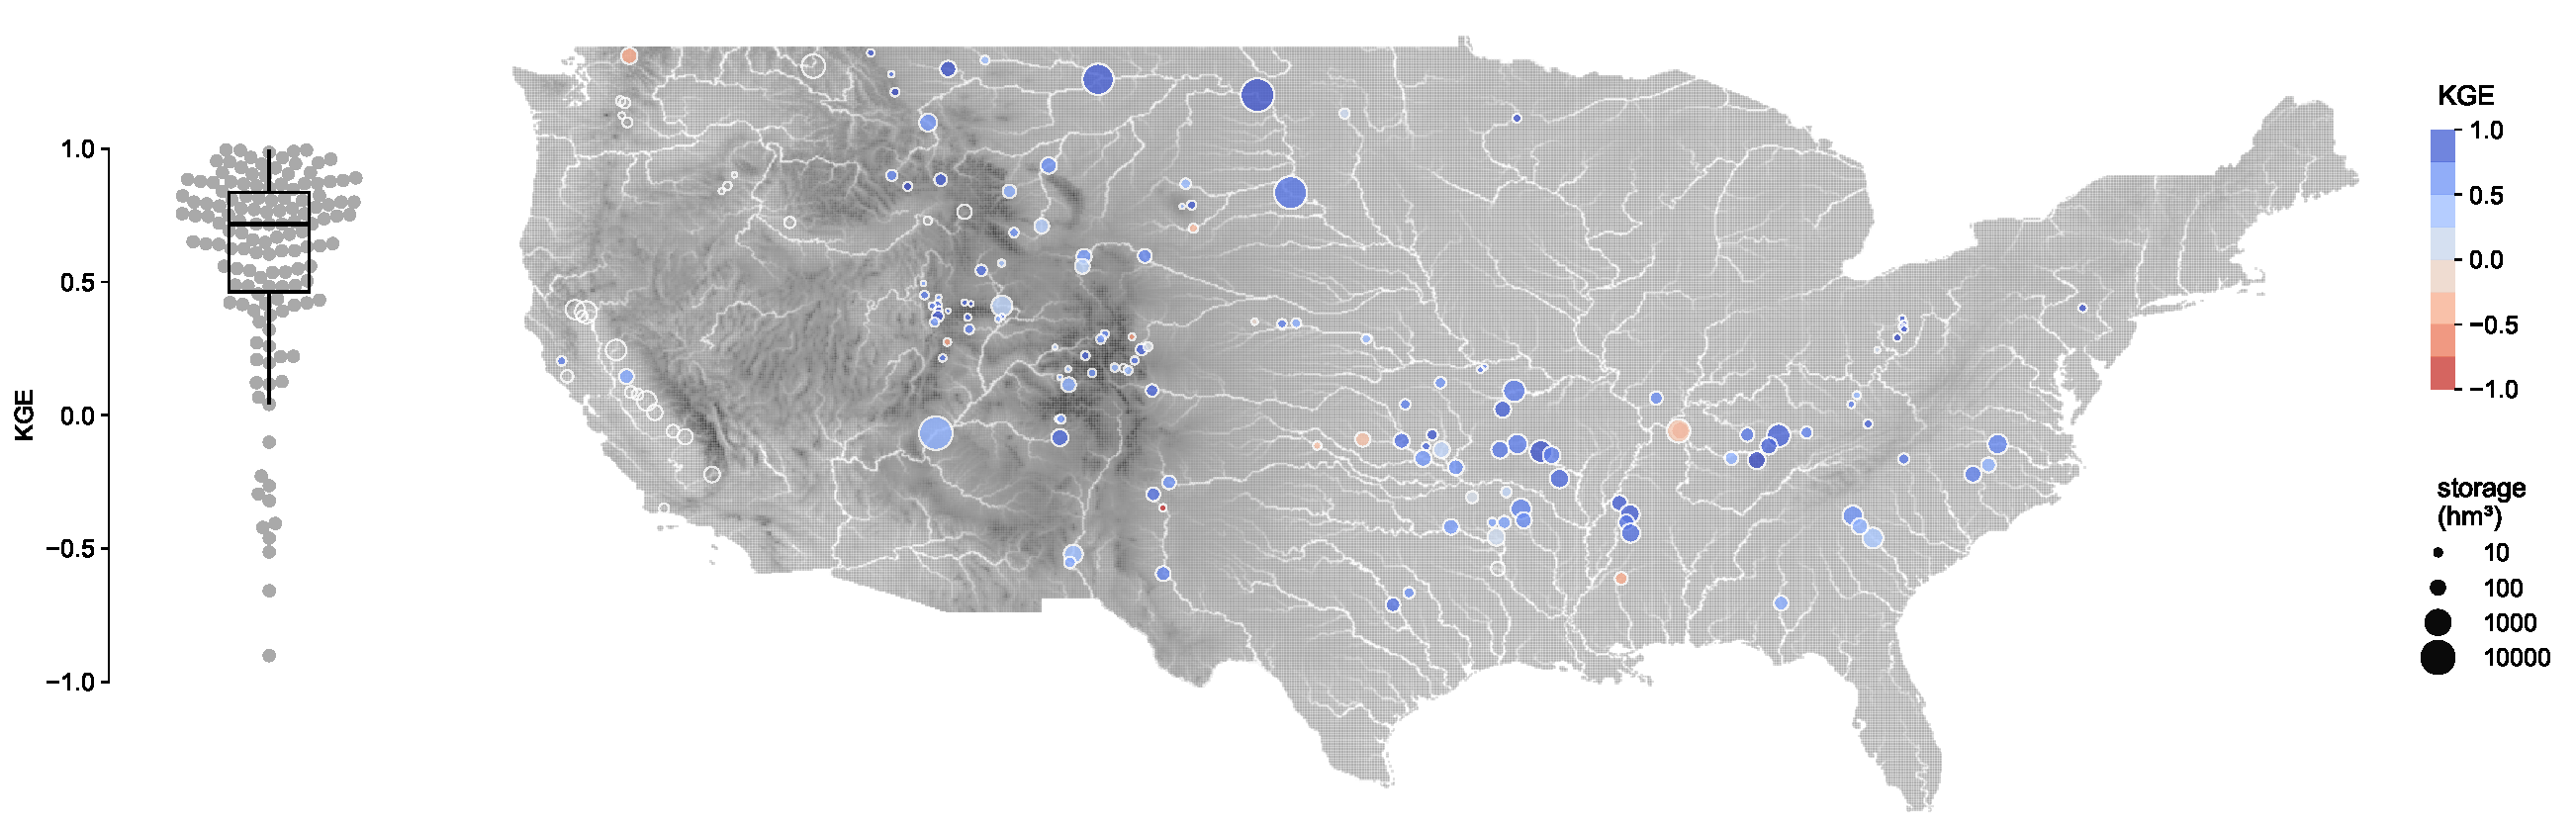
\includegraphics[width=1.0\textwidth]{figures/kge_elevation.pdf}
    \caption{Performance of the reservoir level estimation assuming a half-pyramid reservoir shape. The swarm plot on the left shows the overall distribution, where each point represents a reservoir and the box plot the quartiles. The map on the right shows the geographical distribution of performance; the dot size indicates reservoir storage.}
    \label{fig:elevation_performance}
\end{figure*}

The half-pyramid assumption proved to be a robust approximation for the majority of the study sites. The median KGE' for reservoir level estimation is 0.72, with 75\% of the reservoirs achieving a KGE' at least 0.46. However, the accuracy of the level calculation is highly sensitive to the quality of the static attributes, specifically the crest elevation ($Z_{max}$) and dam height ($H_{dam}$) (see \eqref{eq:level}). As discussed in Section~\ref{sec:reservoir_attributes}, errors in global databases such as GRanD or GDW can propagate into these level estimations; therefore, data cleaning and the use of locally validated attributes are essential for accurate water-level modeling.

\section{Discussion}
\label{sec:discussion}

\subsection{Balancing model complexity and operational feasibility}
\label{sec:comparison_reservoirs}

This study compared reservoir routines of varying complexity, from the simple storage-dependent logic of LISFLOOD to the demand-driven and statistically-inferred policies of mHM and STARFIT. Our results indicate that model performance generally scales with the number of environmental covariates included in the routine (e.g., inflow or demand).

While mHM emerged as the best-performing routine (Section~\ref{sec:compare_models}), its dependence on a demand time series poses a significant operational challenge. In data-rich environments, demand can be inferred via machine learning \citep{Shrestha2024}, but in global systems like EFAS or GloFAS, such data are often unavailable. 

A similar constraint applies to STARFIT, although its performance was not markedly superior to the more parsimonious CaMa-Flood routine. Despite this, STARFIT offers a unique advantage for global regionalization. For instance, \citet{Steyaert2025} recently demonstrated a global application of the STARFIT routine within the PCR-GLOBWB2 hydrological model by leveraging satellite-derived storage from the GloLAKES dataset \citep{Hou2024} to define the storage NOR.

We have selected the CaMa-Flood routine for the implementation in the new version of the LISFLOOD hydrological model that will be the core of the upcoming EFASv6 and GloFASv5 systems. By evolving the current LISFLOOD logic to include inflow-dependency and quadratic storage-outflow relationships, we achieve a measurable gain in performances without increasing the data requirements for calibration. Furthermore, CaMa-Flood's robust default performance makes it an ideal candidate for global applications where historical records are absent.

\subsection{Current limitations and the forecast challenge}
\label{sec:limitations}

A notable limitation across all benchmarked routines is the absence of a explicit use of the reservoir purpose (e.g., irrigation, hydropower, flood control...). While we hypothesize that local calibration allows these routines to learn the specific operations of different reservoir types, the lack of a purpose-aware routine remains a weakness for global modeling.

Furthermore, these routines lack a forward-looking component. In practice, reservoir managers operate based on meteorological and hydrological forecasts across multiple timescales. While replacing current inflow with forecasted inflow as a covariate could address this, it introduces a significant computational bottleneck: the hydrological model would need to simulate the entire upstream catchment for the full forecast horizon before the reservoir release can be determined at any given node.

\subsection{The potential of satellite products}
\label{sec:satellite_products}

The scarcity of in situ records remains the primary hurdle for large-scale reservoir modeling. Satellite-derived products offering reservoir area, elevation, and storage anomalies provide an opportunity to bridge this gap \citep{Zhao2018, Schwatke2020, Donchyts2022, Khandelwal2022, Hou2024}. Two of the outcomes of this study specifically support the transition toward using satellite products. First, we found that reservoir storage is a more informative calibration target than reservoir outflow, as storage-based calibration yields models that perform well across both state variables (Section~\ref{sec:compare_variables}). This represents a "lucky coincidence" for the community, as many available satellite products provide direct estimates of reservoir storage or storage variations rather than discharge. Second, our validation of the inverted half-pyramid shape (Section~\ref{sec:reservoir_shape}) suggests that even simplified geometric assumptions are sufficient to translate satellite-derived levels into volumes with reasonable accuracy.

The flexibility of STARFIT’s harmonic formulation is particularly well-suited for satellite data, as emphasized by \citet{Steyaert2025}. Because the frequency term in the harmonic curves allows the model to be fitted at coarser temporal resolutions (e.g., monthly satellite passes) and then run at a daily time step, it overcomes the temporal sampling limitations of many satellite products.

Furthermore, we have conducted a preliminary analysis of the potential use of the Global Water Watch dataset \citep{Donchyts2022}. Our findings indicate that while satellite-derived storage follows observed historical trends, a persistent bias often exists between in situ and remotely-sensed values. The primary bottleneck for the quality of these products is the availability of accurate elevation-storage-area curves. While several efforts have attempted to provide these curves globally \citep{Yigzaw2018, Busker2019, Khazaei2022}, they frequently show shortcomings when validated against in situ data. This underscores why curated datasets of reservoir operations are so vital: they provide the ground-truth necessary to test and refine these global remotely-sensed approaches.

\subsection{Toward data-driven reservoir modeling}
\label{sec:data-driven}

The recent revolution in deep learning has demonstrated that data-driven models can outperform traditional physical models in streamflow prediction \citep{Nearing2024}. To support this transition in reservoir modeling, we have formatted our ResOpsUS+CARS dataset—along with new national datasets for Brazil \citep{ResOpsBR}, Mexico, and Spain—in the CARAVAN standard.

Reservoir operations are the product of complex human-natural interactions that process-based routines struggle to capture entirely. While we acknowledge that deep learning offers a path toward superior performance, these models are notoriously data-hungry. This highlights the ongoing necessity of curated, multi-national observational datasets—not just for training, but for the rigorous benchmarking of the hybrid physical-statistical models.


\section{Conclusions}
\label{sec:conclusions}

This study provided a comprehensive benchmarking of four reservoir routines (LISFLOOD, CaMa-Flood, mHM, and STARFIT) evaluated across 164 reservoirs in the United States using the ResOpsUS and GRanD datasets. By comparing different calibration strategies and model structures, we draw the following conclusions.

Reservoir storage is the most informative variable for calibration. Our results demonstrate a significant asymmetry in model identifiability. While calibrating routines to match observed outflow (the standard practice in many hydrological models) leads to a poor representation of internal reservoir states, calibrating to storage anomalies yields robust performance for both storage and discharge. This finding supports the shift toward using satellite-derived storage products for model parameterization, particularly in ungauged basins.

mHM offers superior performance, but CaMa-Flood provides the best operational balance. The demand-driven logic of the mHM routine consistently outperformed the other schemes. However, its reliance on site-specific demand data limits its current applicability in global systems like EFAS or GloFAS. The CaMa-Flood routine, which we have now integrated into the LISFLOOD model, represents an optimal compromise: it provides significant improvements over the original linear storage logic without requiring additional input variables or data-intensive calibration.

The half-pyramid geometric assumption is a robust approximation. Validating reservoir level estimations against in situ observations confirmed that a simplified inverted half-pyramid shape is sufficient for large-scale modeling. This validates the use of maximum area and dam height as sufficient proxies to link storage, area, and elevation, which is critical for estimating evaporative losses and integrating altimetry data.

STARFIT’s flexibility is a key asset for remote sensing integration. Although STARFIT did not outperform the rule-based mHM or CaMa-Flood routines in daily simulations, its harmonic formulation is uniquely capable of bridging temporal gaps in observations. Its ability to be fitted at monthly scales and run at daily resolutions makes it a powerful tool for leveraging current and future satellite altimetry missions.

Looking forward, the integration of reservoir modeling into global hydrology must move beyond the "data-poor" paradigm. The creation of standardized, multi-national datasets like the ResOpsUS+CARS and our new national datasets for Brazil, Mexico, and Spain is a step toward this goal. By providing these data in the CARAVAN format, we aim to facilitate the development of hybrid models that combine the physical consistency of process-based routines with the predictive power of deep learning. Such advancements will be essential for improving the accuracy of operational flood and drought forecasting systems in an increasingly managed global water cycle.


\codedataavailability{All the code used to generate the reservoir dataset, implement the four reservoir schemes, and perform the model calibrations is available in the following GitHub repository: \url{https://github.com/casadoj/reservoirs-LSHM}. The benchmarking dataset generated for this study can be accessed via Zenodo at \url{https://doi.org/10.5281/zenodo.15978041}.}

%\appendix

%\noappendix       %% use this to mark the end of the appendix section. Otherwise the figures might be numbered incorrectly (e.g. 10 instead of 1).

%% Regarding figures and tables in appendices, the following two options are possible depending on your general handling of figures and tables in the manuscript environment:

%% Option 1: If you sorted all figures and tables into the sections of the text, please also sort the appendix figures and appendix tables into the respective appendix sections.
%% They will be correctly named automatically.

%% Option 2: If you put all figures after the reference list, please insert appendix tables and figures after the normal tables and figures.
%% To rename them correctly to A1, A2, etc., please add the following commands in front of them:

%\appendixfigures  %% needs to be added in front of appendix figures

%\appendixtables   %% needs to be added in front of appendix tables

%% Please add \clearpage between each table and/or figure. Further guidelines on figures and tables can be found below.



\authorcontribution{TEXT} %% this section is mandatory

\competinginterests{TEXT} %% this section is mandatory even if you declare that no competing interests are present

%\disclaimer{TEXT} %% optional section

\begin{acknowledgements}
TEXT
\end{acknowledgements}


%% REFERENCES

%% The reference list is compiled as follows:

% \begin{thebibliography}{}

% \bibitem[AUTHOR(YEAR)]{LABEL1}
% REFERENCE 1

% \bibitem[AUTHOR(YEAR)]{LABEL2}
% REFERENCE 2

% \end{thebibliography}

%% Since the Copernicus LaTeX package includes the BibTeX style file copernicus.bst,
%% authors experienced with BibTeX only have to include the following two lines:
%%
\bibliographystyle{copernicus}
\bibliography{bibliography.bib}
%%
%% URLs and DOIs can be entered in your BibTeX file as:
%%
%% URL = {http://www.xyz.org/~jones/idx_g.htm}
%% DOI = {10.5194/xyz}


%% LITERATURE CITATIONS
%%
%% command                        & example result
%% \citet{jones90}|               & Jones et al. (1990)
%% \citep{jones90}|               & (Jones et al., 1990)
%% \citep{jones90,jones93}|       & (Jones et al., 1990, 1993)
%% \citep[p.~32]{jones90}|        & (Jones et al., 1990, p.~32)
%% \citep[e.g.,][]{jones90}|      & (e.g., Jones et al., 1990)
%% \citep[e.g.,][p.~32]{jones90}| & (e.g., Jones et al., 1990, p.~32)
%% \citeauthor{jones90}|          & Jones et al.
%% \citeyear{jones90}|            & 1990



%% FIGURES

%% When figures and tables are placed at the end of the MS (article in one-column style), please add \clearpage
%% between bibliography and first table and/or figure as well as between each table and/or figure.

% The figure files should be labelled correctly with Arabic numerals (e.g. fig01.jpg, fig02.png).


%% ONE-COLUMN FIGURES

%%f
%\begin{figure}[t]
%\includegraphics[width=8.3cm]{FILE NAME}
%\caption{TEXT}
%\end{figure}
%
%%% TWO-COLUMN FIGURES
%
%%f
%\begin{figure*}[t]
%\includegraphics[width=12cm]{FILE NAME}
%\caption{TEXT}
%\end{figure*}
%
%
%%% TABLES
%%%
%%% The different columns must be seperated with a & command and should
%%% end with \\ to identify the column brake.
%
%%% ONE-COLUMN TABLE
%
%%t
%\begin{table}[t]
%\caption{TEXT}
%\begin{tabular}{column = lcr}
%\tophline
%
%\middlehline
%
%\bottomhline
%\end{tabular}
%\belowtable{} % Table Footnotes
%\end{table}
%
%%% TWO-COLUMN TABLE
%
%%t
%\begin{table*}[t]
%\caption{TEXT}
%\begin{tabular}{column = lcr}
%\tophline
%
%\middlehline
%
%\bottomhline
%\end{tabular}
%\belowtable{} % Table Footnotes
%\end{table*}
%
%%% LANDSCAPE TABLE
%
%%t
%\begin{sidewaystable*}[t]
%\caption{TEXT}
%\begin{tabular}{column = lcr}
%\tophline
%
%\middlehline
%
%\bottomhline
%\end{tabular}
%\belowtable{} % Table Footnotes
%\end{sidewaystable*}
%
%
%%% MATHEMATICAL EXPRESSIONS
%
%%% All papers typeset by Copernicus Publications follow the math typesetting regulations
%%% given by the IUPAC Green Book (IUPAC: Quantities, Units and Symbols in Physical Chemistry,
%%% 2nd Edn., Blackwell Science, available at: http://old.iupac.org/publications/books/gbook/green_book_2ed.pdf, 1993).
%%%
%%% Physical quantities/variables are typeset in italic font (t for time, T for Temperature)
%%% Indices which are not defined are typeset in italic font (x, y, z, a, b, c)
%%% Items/objects which are defined are typeset in roman font (Car A, Car B)
%%% Descriptions/specifications which are defined by itself are typeset in roman font (abs, rel, ref, tot, net, ice)
%%% Abbreviations from 2 letters are typeset in roman font (RH, LAI)
%%% Vectors are identified in bold italic font using \vec{x}
%%% Matrices are identified in bold roman font
%%% Multiplication signs are typeset using the LaTeX commands \times (for vector products, grids, and exponential notations) or \cdot
%%% The character * should not be applied as mutliplication sign
%
%
%%% EQUATIONS
%
%%% Single-row equation
%
%\begin{equation}
%
%\end{equation}
%
%%% Multiline equation
%
%\begin{align}
%& 3 + 5 = 8\\
%& 3 + 5 = 8\\
%& 3 + 5 = 8
%\end{align}
%
%
%%% MATRICES
%
%\begin{matrix}
%x & y & z\\
%x & y & z\\
%x & y & z\\
%\end{matrix}
%
%
%%% ALGORITHM
%
%\begin{algorithm}
%\caption{...}
%\label{a1}
%\begin{algorithmic}
%...
%\end{algorithmic}
%\end{algorithm}
%
%
%%% CHEMICAL FORMULAS AND REACTIONS
%
%%% For formulas embedded in the text, please use \chem{}
%
%%% The reaction environment creates labels including the letter R, i.e. (R1), (R2), etc.
%
%\begin{reaction}
%%% \rightarrow should be used for normal (one-way) chemical reactions
%%% \rightleftharpoons should be used for equilibria
%%% \leftrightarrow should be used for resonance structures
%\end{reaction}
%
%
%%% PHYSICAL UNITS
%%%
%%% Please use \unit{} and apply the exponential notation


\end{document}
